% Options for packages loaded elsewhere
\PassOptionsToPackage{unicode}{hyperref}
\PassOptionsToPackage{hyphens}{url}
\PassOptionsToPackage{dvipsnames,svgnames,x11names}{xcolor}
%
\documentclass[
  letterpaper,
  DIV=11,
  numbers=noendperiod]{scrartcl}

\usepackage{amsmath,amssymb}
\usepackage{lmodern}
\usepackage{iftex}
\ifPDFTeX
  \usepackage[T1]{fontenc}
  \usepackage[utf8]{inputenc}
  \usepackage{textcomp} % provide euro and other symbols
\else % if luatex or xetex
  \usepackage{unicode-math}
  \defaultfontfeatures{Scale=MatchLowercase}
  \defaultfontfeatures[\rmfamily]{Ligatures=TeX,Scale=1}
\fi
% Use upquote if available, for straight quotes in verbatim environments
\IfFileExists{upquote.sty}{\usepackage{upquote}}{}
\IfFileExists{microtype.sty}{% use microtype if available
  \usepackage[]{microtype}
  \UseMicrotypeSet[protrusion]{basicmath} % disable protrusion for tt fonts
}{}
\makeatletter
\@ifundefined{KOMAClassName}{% if non-KOMA class
  \IfFileExists{parskip.sty}{%
    \usepackage{parskip}
  }{% else
    \setlength{\parindent}{0pt}
    \setlength{\parskip}{6pt plus 2pt minus 1pt}}
}{% if KOMA class
  \KOMAoptions{parskip=half}}
\makeatother
\usepackage{xcolor}
\setlength{\emergencystretch}{3em} % prevent overfull lines
\setcounter{secnumdepth}{-\maxdimen} % remove section numbering
% Make \paragraph and \subparagraph free-standing
\ifx\paragraph\undefined\else
  \let\oldparagraph\paragraph
  \renewcommand{\paragraph}[1]{\oldparagraph{#1}\mbox{}}
\fi
\ifx\subparagraph\undefined\else
  \let\oldsubparagraph\subparagraph
  \renewcommand{\subparagraph}[1]{\oldsubparagraph{#1}\mbox{}}
\fi

\usepackage{color}
\usepackage{fancyvrb}
\newcommand{\VerbBar}{|}
\newcommand{\VERB}{\Verb[commandchars=\\\{\}]}
\DefineVerbatimEnvironment{Highlighting}{Verbatim}{commandchars=\\\{\}}
% Add ',fontsize=\small' for more characters per line
\usepackage{framed}
\definecolor{shadecolor}{RGB}{241,243,245}
\newenvironment{Shaded}{\begin{snugshade}}{\end{snugshade}}
\newcommand{\AlertTok}[1]{\textcolor[rgb]{0.68,0.00,0.00}{#1}}
\newcommand{\AnnotationTok}[1]{\textcolor[rgb]{0.37,0.37,0.37}{#1}}
\newcommand{\AttributeTok}[1]{\textcolor[rgb]{0.40,0.45,0.13}{#1}}
\newcommand{\BaseNTok}[1]{\textcolor[rgb]{0.68,0.00,0.00}{#1}}
\newcommand{\BuiltInTok}[1]{\textcolor[rgb]{0.00,0.23,0.31}{#1}}
\newcommand{\CharTok}[1]{\textcolor[rgb]{0.13,0.47,0.30}{#1}}
\newcommand{\CommentTok}[1]{\textcolor[rgb]{0.37,0.37,0.37}{#1}}
\newcommand{\CommentVarTok}[1]{\textcolor[rgb]{0.37,0.37,0.37}{\textit{#1}}}
\newcommand{\ConstantTok}[1]{\textcolor[rgb]{0.56,0.35,0.01}{#1}}
\newcommand{\ControlFlowTok}[1]{\textcolor[rgb]{0.00,0.23,0.31}{#1}}
\newcommand{\DataTypeTok}[1]{\textcolor[rgb]{0.68,0.00,0.00}{#1}}
\newcommand{\DecValTok}[1]{\textcolor[rgb]{0.68,0.00,0.00}{#1}}
\newcommand{\DocumentationTok}[1]{\textcolor[rgb]{0.37,0.37,0.37}{\textit{#1}}}
\newcommand{\ErrorTok}[1]{\textcolor[rgb]{0.68,0.00,0.00}{#1}}
\newcommand{\ExtensionTok}[1]{\textcolor[rgb]{0.00,0.23,0.31}{#1}}
\newcommand{\FloatTok}[1]{\textcolor[rgb]{0.68,0.00,0.00}{#1}}
\newcommand{\FunctionTok}[1]{\textcolor[rgb]{0.28,0.35,0.67}{#1}}
\newcommand{\ImportTok}[1]{\textcolor[rgb]{0.00,0.46,0.62}{#1}}
\newcommand{\InformationTok}[1]{\textcolor[rgb]{0.37,0.37,0.37}{#1}}
\newcommand{\KeywordTok}[1]{\textcolor[rgb]{0.00,0.23,0.31}{#1}}
\newcommand{\NormalTok}[1]{\textcolor[rgb]{0.00,0.23,0.31}{#1}}
\newcommand{\OperatorTok}[1]{\textcolor[rgb]{0.37,0.37,0.37}{#1}}
\newcommand{\OtherTok}[1]{\textcolor[rgb]{0.00,0.23,0.31}{#1}}
\newcommand{\PreprocessorTok}[1]{\textcolor[rgb]{0.68,0.00,0.00}{#1}}
\newcommand{\RegionMarkerTok}[1]{\textcolor[rgb]{0.00,0.23,0.31}{#1}}
\newcommand{\SpecialCharTok}[1]{\textcolor[rgb]{0.37,0.37,0.37}{#1}}
\newcommand{\SpecialStringTok}[1]{\textcolor[rgb]{0.13,0.47,0.30}{#1}}
\newcommand{\StringTok}[1]{\textcolor[rgb]{0.13,0.47,0.30}{#1}}
\newcommand{\VariableTok}[1]{\textcolor[rgb]{0.07,0.07,0.07}{#1}}
\newcommand{\VerbatimStringTok}[1]{\textcolor[rgb]{0.13,0.47,0.30}{#1}}
\newcommand{\WarningTok}[1]{\textcolor[rgb]{0.37,0.37,0.37}{\textit{#1}}}

\providecommand{\tightlist}{%
  \setlength{\itemsep}{0pt}\setlength{\parskip}{0pt}}\usepackage{longtable,booktabs,array}
\usepackage{calc} % for calculating minipage widths
% Correct order of tables after \paragraph or \subparagraph
\usepackage{etoolbox}
\makeatletter
\patchcmd\longtable{\par}{\if@noskipsec\mbox{}\fi\par}{}{}
\makeatother
% Allow footnotes in longtable head/foot
\IfFileExists{footnotehyper.sty}{\usepackage{footnotehyper}}{\usepackage{footnote}}
\makesavenoteenv{longtable}
\usepackage{graphicx}
\makeatletter
\def\maxwidth{\ifdim\Gin@nat@width>\linewidth\linewidth\else\Gin@nat@width\fi}
\def\maxheight{\ifdim\Gin@nat@height>\textheight\textheight\else\Gin@nat@height\fi}
\makeatother
% Scale images if necessary, so that they will not overflow the page
% margins by default, and it is still possible to overwrite the defaults
% using explicit options in \includegraphics[width, height, ...]{}
\setkeys{Gin}{width=\maxwidth,height=\maxheight,keepaspectratio}
% Set default figure placement to htbp
\makeatletter
\def\fps@figure{htbp}
\makeatother
\newlength{\cslhangindent}
\setlength{\cslhangindent}{1.5em}
\newlength{\csllabelwidth}
\setlength{\csllabelwidth}{3em}
\newlength{\cslentryspacingunit} % times entry-spacing
\setlength{\cslentryspacingunit}{\parskip}
\newenvironment{CSLReferences}[2] % #1 hanging-ident, #2 entry spacing
 {% don't indent paragraphs
  \setlength{\parindent}{0pt}
  % turn on hanging indent if param 1 is 1
  \ifodd #1
  \let\oldpar\par
  \def\par{\hangindent=\cslhangindent\oldpar}
  \fi
  % set entry spacing
  \setlength{\parskip}{#2\cslentryspacingunit}
 }%
 {}
\usepackage{calc}
\newcommand{\CSLBlock}[1]{#1\hfill\break}
\newcommand{\CSLLeftMargin}[1]{\parbox[t]{\csllabelwidth}{#1}}
\newcommand{\CSLRightInline}[1]{\parbox[t]{\linewidth - \csllabelwidth}{#1}\break}
\newcommand{\CSLIndent}[1]{\hspace{\cslhangindent}#1}

\usepackage{booktabs}
\usepackage{longtable}
\usepackage{array}
\usepackage{multirow}
\usepackage{wrapfig}
\usepackage{float}
\usepackage{colortbl}
\usepackage{pdflscape}
\usepackage{tabu}
\usepackage{threeparttable}
\usepackage{threeparttablex}
\usepackage[normalem]{ulem}
\usepackage{makecell}
\usepackage{xcolor}
\KOMAoption{captions}{tableheading}
\makeatletter
\makeatother
\makeatletter
\makeatother
\makeatletter
\@ifpackageloaded{caption}{}{\usepackage{caption}}
\AtBeginDocument{%
\ifdefined\contentsname
  \renewcommand*\contentsname{Table of contents}
\else
  \newcommand\contentsname{Table of contents}
\fi
\ifdefined\listfigurename
  \renewcommand*\listfigurename{List of Figures}
\else
  \newcommand\listfigurename{List of Figures}
\fi
\ifdefined\listtablename
  \renewcommand*\listtablename{List of Tables}
\else
  \newcommand\listtablename{List of Tables}
\fi
\ifdefined\figurename
  \renewcommand*\figurename{Figure}
\else
  \newcommand\figurename{Figure}
\fi
\ifdefined\tablename
  \renewcommand*\tablename{Table}
\else
  \newcommand\tablename{Table}
\fi
}
\@ifpackageloaded{float}{}{\usepackage{float}}
\floatstyle{ruled}
\@ifundefined{c@chapter}{\newfloat{codelisting}{h}{lop}}{\newfloat{codelisting}{h}{lop}[chapter]}
\floatname{codelisting}{Listing}
\newcommand*\listoflistings{\listof{codelisting}{List of Listings}}
\makeatother
\makeatletter
\@ifpackageloaded{caption}{}{\usepackage{caption}}
\@ifpackageloaded{subcaption}{}{\usepackage{subcaption}}
\makeatother
\makeatletter
\@ifpackageloaded{tcolorbox}{}{\usepackage[many]{tcolorbox}}
\makeatother
\makeatletter
\@ifundefined{shadecolor}{\definecolor{shadecolor}{rgb}{.97, .97, .97}}
\makeatother
\makeatletter
\makeatother
\ifLuaTeX
  \usepackage{selnolig}  % disable illegal ligatures
\fi
\IfFileExists{bookmark.sty}{\usepackage{bookmark}}{\usepackage{hyperref}}
\IfFileExists{xurl.sty}{\usepackage{xurl}}{} % add URL line breaks if available
\urlstyle{same} % disable monospaced font for URLs
\hypersetup{
  pdftitle={Quarto dokument},
  colorlinks=true,
  linkcolor={blue},
  filecolor={Maroon},
  citecolor={Blue},
  urlcolor={Blue},
  pdfcreator={LaTeX via pandoc}}

\title{Quarto dokument}
\author{}
\date{}

\begin{document}
\maketitle
\ifdefined\Shaded\renewenvironment{Shaded}{\begin{tcolorbox}[borderline west={3pt}{0pt}{shadecolor}, enhanced, interior hidden, frame hidden, boxrule=0pt, sharp corners, breakable]}{\end{tcolorbox}}\fi

\begin{Shaded}
\begin{Highlighting}[]
\FunctionTok{library}\NormalTok{(tidyverse)}
\FunctionTok{library}\NormalTok{(kableExtra)}
\end{Highlighting}
\end{Shaded}

\hypertarget{overskrift}{%
\subsection{Overskrift}\label{overskrift}}

Vanlig brødtekst før vi har en «code chunck»

\begin{Shaded}
\begin{Highlighting}[]
\DecValTok{2} \SpecialCharTok{+} \DecValTok{2}
\end{Highlighting}
\end{Shaded}

\begin{verbatim}
[1] 4
\end{verbatim}

og forsetter med en ny der vi definerer en variabel.

\begin{Shaded}
\begin{Highlighting}[]
\NormalTok{x }\OtherTok{\textless{}{-}} \DecValTok{3} \SpecialCharTok{+} \DecValTok{3} \SpecialCharTok{+} \FunctionTok{log}\NormalTok{(}\DecValTok{10}\NormalTok{)}
\end{Highlighting}
\end{Shaded}

Henter inn et eksempel datasett:

\begin{Shaded}
\begin{Highlighting}[]
\FunctionTok{data}\NormalTok{(mtcars)}
\end{Highlighting}
\end{Shaded}

Sjekker toppen av \texttt{mtcars}. Se output fra code-chunk under.

\begin{Shaded}
\begin{Highlighting}[]
\FunctionTok{head}\NormalTok{(mtcars, }\AttributeTok{n =} \DecValTok{5}\NormalTok{)}
\end{Highlighting}
\end{Shaded}

\begin{verbatim}
                   mpg cyl disp  hp drat    wt  qsec vs am gear carb
Mazda RX4         21.0   6  160 110 3.90 2.620 16.46  0  1    4    4
Mazda RX4 Wag     21.0   6  160 110 3.90 2.875 17.02  0  1    4    4
Datsun 710        22.8   4  108  93 3.85 2.320 18.61  1  1    4    1
Hornet 4 Drive    21.4   6  258 110 3.08 3.215 19.44  1  0    3    1
Hornet Sportabout 18.7   8  360 175 3.15 3.440 17.02  0  0    3    2
\end{verbatim}

Vi kan også generere fint formaterte tabeller som den i
Table~\ref{tbl-fem_første_mtcars}.

\begin{Shaded}
\begin{Highlighting}[]
\FunctionTok{head}\NormalTok{(mtcars, }\AttributeTok{n =} \DecValTok{5}\NormalTok{) }\SpecialCharTok{|\textgreater{}}
  \FunctionTok{kbl}\NormalTok{(}\AttributeTok{booktabs =}\NormalTok{ T) }\SpecialCharTok{|\textgreater{}}
  \FunctionTok{kable\_styling}\NormalTok{(}\AttributeTok{latex\_options =} \FunctionTok{c}\NormalTok{(}\StringTok{"HOLD\_position"}\NormalTok{, }\StringTok{"striped"}\NormalTok{),}
                \AttributeTok{full\_width =}\NormalTok{ F, }\AttributeTok{font\_size =} \DecValTok{8}\NormalTok{)}
\end{Highlighting}
\end{Shaded}

\hypertarget{tbl-fem_fuxf8rste_mtcars}{}
\begin{table}[H]
\caption{\label{tbl-fem_første_mtcars}Fem første rekkene i mtcars. Satt med font\_size = 8. }\tabularnewline

\centering\begingroup\fontsize{8}{10}\selectfont

\begin{tabular}[t]{lrrrrrrrrrrr}
\toprule
  & mpg & cyl & disp & hp & drat & wt & qsec & vs & am & gear & carb\\
\midrule
\cellcolor{gray!6}{Mazda RX4} & \cellcolor{gray!6}{21.0} & \cellcolor{gray!6}{6} & \cellcolor{gray!6}{160} & \cellcolor{gray!6}{110} & \cellcolor{gray!6}{3.90} & \cellcolor{gray!6}{2.620} & \cellcolor{gray!6}{16.46} & \cellcolor{gray!6}{0} & \cellcolor{gray!6}{1} & \cellcolor{gray!6}{4} & \cellcolor{gray!6}{4}\\
Mazda RX4 Wag & 21.0 & 6 & 160 & 110 & 3.90 & 2.875 & 17.02 & 0 & 1 & 4 & 4\\
\cellcolor{gray!6}{Datsun 710} & \cellcolor{gray!6}{22.8} & \cellcolor{gray!6}{4} & \cellcolor{gray!6}{108} & \cellcolor{gray!6}{93} & \cellcolor{gray!6}{3.85} & \cellcolor{gray!6}{2.320} & \cellcolor{gray!6}{18.61} & \cellcolor{gray!6}{1} & \cellcolor{gray!6}{1} & \cellcolor{gray!6}{4} & \cellcolor{gray!6}{1}\\
Hornet 4 Drive & 21.4 & 6 & 258 & 110 & 3.08 & 3.215 & 19.44 & 1 & 0 & 3 & 1\\
\cellcolor{gray!6}{Hornet Sportabout} & \cellcolor{gray!6}{18.7} & \cellcolor{gray!6}{8} & \cellcolor{gray!6}{360} & \cellcolor{gray!6}{175} & \cellcolor{gray!6}{3.15} & \cellcolor{gray!6}{3.440} & \cellcolor{gray!6}{17.02} & \cellcolor{gray!6}{0} & \cellcolor{gray!6}{0} & \cellcolor{gray!6}{3} & \cellcolor{gray!6}{2}\\
\bottomrule
\end{tabular}
\endgroup{}
\end{table}

Hvis vi bare vil ha tabellen og ikke koden som genererer den endrer vi
til:

\begin{figure}

{\centering 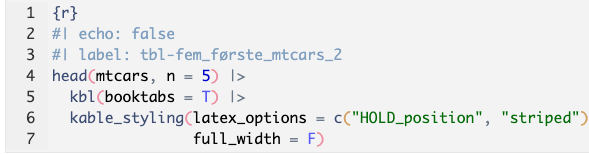
\includegraphics{echo-false.png}

}

\caption{\label{fig-echo_false}Dette er et bilde av en Code-chunk» dere
echo: false er satt slik at koden ikke vises.}

\end{figure}

Resultatet av koden i Figure~\ref{fig-echo_false} ovenfor er tabellen
gjengitt i Table~\ref{tbl-fem_første_mtcars_2}.

\hypertarget{tbl-fem_fuxf8rste_mtcars_2}{}
\begin{table}[H]
\caption{\label{tbl-fem_første_mtcars_2}De fem første linjene fra mtcars som formatert tabell. Nå med normal
font størrelse. }\tabularnewline

\centering
\begin{tabular}[t]{lrrrrrrrrrrr}
\toprule
  & mpg & cyl & disp & hp & drat & wt & qsec & vs & am & gear & carb\\
\midrule
\cellcolor{gray!6}{Mazda RX4} & \cellcolor{gray!6}{21.0} & \cellcolor{gray!6}{6} & \cellcolor{gray!6}{160} & \cellcolor{gray!6}{110} & \cellcolor{gray!6}{3.90} & \cellcolor{gray!6}{2.620} & \cellcolor{gray!6}{16.46} & \cellcolor{gray!6}{0} & \cellcolor{gray!6}{1} & \cellcolor{gray!6}{4} & \cellcolor{gray!6}{4}\\
Mazda RX4 Wag & 21.0 & 6 & 160 & 110 & 3.90 & 2.875 & 17.02 & 0 & 1 & 4 & 4\\
\cellcolor{gray!6}{Datsun 710} & \cellcolor{gray!6}{22.8} & \cellcolor{gray!6}{4} & \cellcolor{gray!6}{108} & \cellcolor{gray!6}{93} & \cellcolor{gray!6}{3.85} & \cellcolor{gray!6}{2.320} & \cellcolor{gray!6}{18.61} & \cellcolor{gray!6}{1} & \cellcolor{gray!6}{1} & \cellcolor{gray!6}{4} & \cellcolor{gray!6}{1}\\
Hornet 4 Drive & 21.4 & 6 & 258 & 110 & 3.08 & 3.215 & 19.44 & 1 & 0 & 3 & 1\\
\cellcolor{gray!6}{Hornet Sportabout} & \cellcolor{gray!6}{18.7} & \cellcolor{gray!6}{8} & \cellcolor{gray!6}{360} & \cellcolor{gray!6}{175} & \cellcolor{gray!6}{3.15} & \cellcolor{gray!6}{3.440} & \cellcolor{gray!6}{17.02} & \cellcolor{gray!6}{0} & \cellcolor{gray!6}{0} & \cellcolor{gray!6}{3} & \cellcolor{gray!6}{2}\\
\bottomrule
\end{tabular}
\end{table}

Alle objekter vi har definert dukker opp i \textbf{Environment} fanen i
øvre høyre hjørne. Se figur Figure~\ref{fig-env}.

\begin{figure}

{\centering 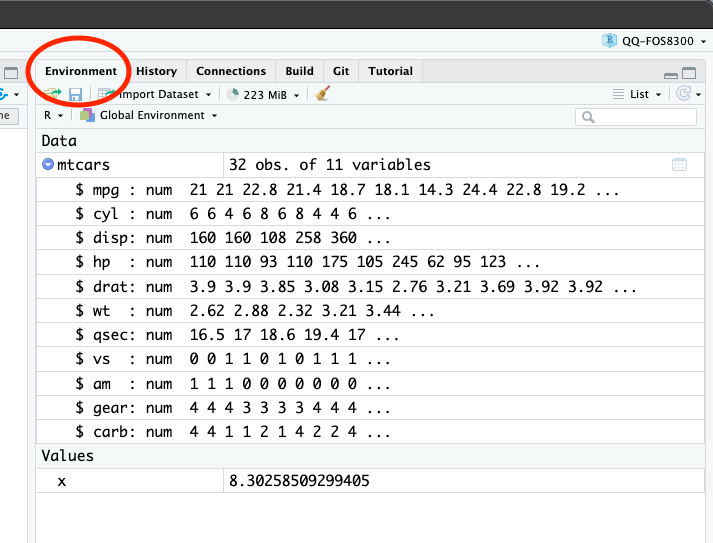
\includegraphics{Env.png}

}

\caption{\label{fig-env}Objekter definert i gjeldene «namespace».}

\end{figure}

Mer om Quarto dokumenter finner en i {``R for {Data Science} (2e) - 30~
{Quarto}''} (n.d.). God og oppdatert informasjon om \texttt{tidyverse}
finner man på sidene {``Easily {Install} and {Load} the {Tidyverse}''}
(n.d.).

\hypertarget{referanser}{%
\subsection{Referanser}\label{referanser}}

\hypertarget{refs}{}
\begin{CSLReferences}{1}{0}
\leavevmode\vadjust pre{\hypertarget{ref-zotero-1459}{}}%
{``Easily {Install} and {Load} the {Tidyverse}.''} n.d.
\url{https://tidyverse.tidyverse.org/}.

\leavevmode\vadjust pre{\hypertarget{ref-zotero-1457}{}}%
{``R for {Data Science} (2e) - 30~ {Quarto}.''} n.d.
\url{https://r4ds.hadley.nz/quarto.html}.

\end{CSLReferences}

\hypertarget{appendiks}{%
\subsection{Appendiks}\label{appendiks}}

Resultat av kommandoen sessionInfo(). Det siste her mest for å vise
hvordan man får plassert referanselisten før appendikset.

\begin{verbatim}
> sessionInfo() |> print(width = 78)
R version 4.2.2 (2022-10-31)
Platform: aarch64-apple-darwin20 (64-bit)
Running under: macOS Monterey 12.5.1

Matrix products: default
LAPACK: /Library/Frameworks/R.framework/Versions/4.2-arm64/Resources/lib/libRlapack.dylib

locale:
[1] en_US.UTF-8/en_US.UTF-8/en_US.UTF-8/C/en_US.UTF-8/en_US.UTF-8

attached base packages:
[1] stats     graphics  grDevices datasets  utils     methods   base     

other attached packages:
 [1] kableExtra_1.3.4   forcats_0.5.2      stringr_1.5.0.9000
 [4] dplyr_1.0.10       purrr_0.3.5        readr_2.1.3       
 [7] tidyr_1.2.1        tibble_3.1.8       ggplot2_3.4.0     
[10] tidyverse_1.3.2   

loaded via a namespace (and not attached):
 [1] gert_1.9.2          svglite_2.1.0       lubridate_1.9.0    
 [4] gitcreds_0.1.2      assertthat_0.2.1    rprojroot_2.0.3    
 [7] digest_0.6.29       utf8_1.2.2          R6_2.5.1           
[10] cellranger_1.1.0    backports_1.4.1     sys_3.4.1          
[13] reprex_2.0.2        evaluate_0.16       highr_0.9          
[16] httr_1.4.4          pillar_1.8.1        rlang_1.0.6        
[19] googlesheets4_1.0.1 curl_4.3.3          readxl_1.4.1       
[22] rstudioapi_0.14     jquerylib_0.1.4     rmarkdown_2.15     
[25] webshot_0.5.4       googledrive_2.0.0   munsell_0.5.0      
[28] broom_1.0.2         compiler_4.2.2      modelr_0.1.10      
[31] xfun_0.32           systemfonts_1.0.4   pkgconfig_2.0.3    
[34] askpass_1.1         htmltools_0.5.3     openssl_2.0.5      
[37] tidyselect_1.2.0    viridisLite_0.4.1   fansi_1.0.3        
[40] crayon_1.5.2        tzdb_0.3.0          dbplyr_2.2.1       
[43] withr_2.5.0         grid_4.2.2          jsonlite_1.8.0     
[46] gtable_0.3.1        lifecycle_1.0.3     DBI_1.1.3          
[49] magrittr_2.0.3      credentials_1.3.2   scales_1.2.1       
[52] cachem_1.0.6        cli_3.4.1           stringi_1.7.8      
[55] renv_0.15.5         fs_1.5.2            bslib_0.4.0        
[58] xml2_1.3.3          ellipsis_0.3.2      generics_0.1.3     
[61] vctrs_0.5.1         gh_1.3.1            tools_4.2.2        
[64] glue_1.6.2          hms_1.1.2           fastmap_1.1.0      
[67] timechange_0.1.1    colorspace_2.0-3    gargle_1.2.1       
[70] rvest_1.0.3         knitr_1.39          haven_2.5.1        
[73] sass_0.4.2          usethis_2.1.6      
> 
\end{verbatim}



\end{document}
